%--------------------------------------------------------------------------
%-------------------------------------------------------------------------------
\subsection{Botafumeiro}
%--------------------------------------------------------------------------
%--------------------------------------------------------------------------
\begin{minipage}[c]{.60\linewidth}
Nous allons modéliser le {\bf botafumeiro}, c'est un encensoir de la cathédrale de Saint-Jacques-de-Compostelle fixé par une poulie sur le plafond et animé par une excitation  humaine ;  des prêtres raccourcissent la longueur du pendule lors des remontées et relâchent la corde lors des descentes.
\end{minipage}  
%--------------------------------------------------------------------------
\begin{minipage}[c]{.40\linewidth}
\begin{center}
\begin{tikzpicture}
\draw[dashed] (0,0) node[above left] {Poulie de petit rayon} -- (0, -5);
\draw[fill] (0, 0) circle (0.1);
\draw (30:0.05)  -- (-60:5);
\draw[fill] (-60:5) circle (0.2);
\draw (165:0.05)  -- (255:4.5);
\draw[<->] (245:3)  -- +(75:1);
\node[priest,minimum size=1.5cm] (B) at (250:4.5) {};
\end{tikzpicture}  
\end{center}
\end{minipage}  
%--------------------------------------------------------------------------
On note $l(t)$ la longueur de cette corde. L'équation régissant le mouvement devient
\[
l(t)\cdot\frac{\d^2 \theta}{\d t^2} + 
\underbrace{\left(\frac{\alpha}m\cdot l(t) + 2 \cdot\frac{\d l}{\d t}\right)}_{\lambda}
\cdot\frac{\d \theta}{\d t} + g.\sin(\theta) = 0
\]

$\alpha$ est le coefficient de frottement (que l'on pourra négliger)et $m$ est la masse de l'encensoir.

Généralement, le coefficient $\lambda$ est positif et amène à une décroissance exponentielle dans le cas d’une équation à coefficients constants due aux amortissements. Par contre, si ce terme est négatif, on aura, au contraire, une augmentation de l’amplitude due à l’apport d’énergie du moteur. Si on oublie les frottements, ce terme est négatif si $l(t)$ diminue dont si on tire sur la corde. Cela correspond à un apport d’énergie par les personnes qui tirent la corde du botafumeiro, et cet apport d’énergie se traduit par une augmentation de l’amplitude des oscillations. Mais pour que la corde puisse être raccourcie, il faut également l’allonger! Dans un cycle d’oscillation, il faut donc "pomper", en choisissant le moment opportun pour allonger ou raccourcir la corde. Expérimentalement on voit que le maximum d’efficacité s’obtient si on tire quand la corde est à la verticale, et qu’on la relâche quand la vitesse s’annule (deux cycles de pompage par période).

%--------------------------------------------------------------------------
\begin{minipage}[c]{.40\linewidth}
Nous allons simplifier l'action humaine en la remplaçant par un moteur  tournant à la vitesse de rotation $\Omega$ qui  modifie la longueur de la corde du pendule de sorte qu'elle vérifie 
$l(t) = l_0 + a \sin(\Omega t)$.


On prendra $m = 60\text{kg}$, $g = 9,81\text{m}\cdot\text{s}^{-2}$, $l_0 = 65\text{m}$, $a = 10\text{m}$.

On rappelle qu'on néglige le coefficient d'amortissement $\alpha$.

On note $\omega_0 =\sqrt{g/l_0}$.
\end{minipage}  
%--------------------------------------------------------------------------
\begin{minipage}[c]{.60\linewidth}
\begin{center}
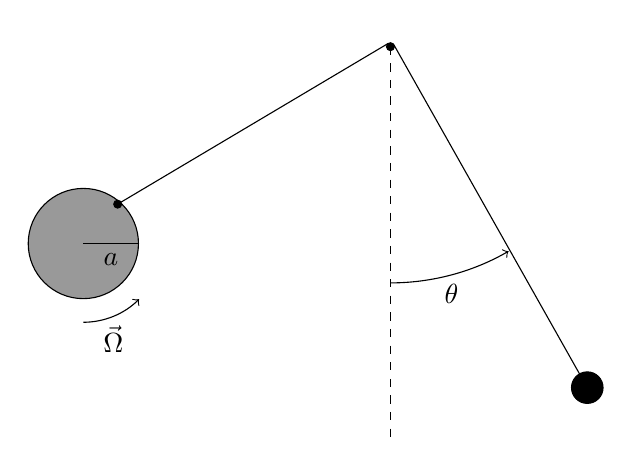
\begin{tikzpicture}
\draw[dashed] (0,0) node[above left] {} -- (0, -5);
\draw[fill] (0, 0) circle (0.05);
\draw (30:0.05)  -- (-60:5);
\draw[->] (0, -3) arc (-90:-60:3) node [midway, below] {$\theta$};
\draw[fill] (-60:5) circle (0.2);
\draw (120:0.05)  -- (210:4);
\draw[fill=gray!80] (-3.9, -2.5) circle (0.7);
\draw[fill] (210:4) circle (0.05);
\draw (-3.9, -2.5) -- node[below] {$a$} (-3.2, -2.5);
\draw[->] (-3.9, -3.5) arc (-90:-45:1) node [midway, below] {$\vec \Omega$};
% \draw[dotted,->] (0,0) -- (0, -4.5) node [below]{$x$};
% \draw[dotted,->] (0,0) -- (3.5, 0) node [right]{$y$};
% \draw[fill] (2.1, -2.8) circle (0.09);
% \draw[->] (0, -1) arc (-90:-53:1) node [midway, below] {$\theta$};
% \draw[dotted] (0, -3.5) arc (-90:-25:3.5) ;
% \draw[very thick, ->] (2.1, -2.8) -- node [left] {$m\overrightarrow g$} +(0, -1.5);
% \draw[very thick, ->] (2.1, -2.8) -- node [above right] {$\overrightarrow R(\theta)$} +(-0.72, 0.96);
% \draw[->] (2.1, -2.8) -- +(0.6, -0.8) node [right] {$\overrightarrow{u_r}$};
% \draw[->] (2.1, -2.8) -- +(0.8,  0.6) node [right] {$\overrightarrow{u_\theta}$};
% %\draw[->] (2.1, -2.8) -- node [above right] {$\vec a$} +(-0.72, -0.54);
\end{tikzpicture}  
\end{center}
\end{minipage}  
